% state-of-the-art_straka.tex
%
% Drafted by Juntang on August 22, 2024
% 

\begin{frame}
  \frametitle{State of the Art (II)}
  \cite{strakaRealTimeDiffusion2010}
    \begin{columns}[T]
    \begin{column}{0.55\textwidth}
    {\small
    \begin{enumerate}
        \item $C_{AIF} \rightarrow (C_{in}) \rightarrow C_{tissue}$:
        \begin{equation}
            \small
            C_{tissue}(t) = \left( C_{AIF} * R_{1\&2}^{[S]} \right)(t)
        \end{equation}
        \begin{equation}
            \small
            R_{1\&2}^{[S]}(t) = \frac{1}{TR}FT^{-1}\{g(f)\frac{c_t(f)}{c_a(f)}\}
        \end{equation}
        
        \item[] where:
        $\begin{aligned}
            c_t(f) &= FT\{C_{tissue}'(t)\} \\
            c_a(f) &= FT\{C_{AIF}'(t)\} \\
            g(f) &= {\left\{
            \begin{array}{lll}
            \frac{c_a(f)^2-N^2}{c_a(f)^2} & \text{if } c_a(f)>N, f\neq0 \\
            1 & \text{if } f=0 \\
            0 & \text{otherwise}
            \end{array}
            \right.}
        \end{aligned}$  
         {\tiny $TR$ is sampling rate, $FT{}$ denotes Fourier Transform, and $'$ denotes signal zero padded.}
    \end{enumerate}
    }
    \end{column}
    
    \hspace*{4em}                                                          %%  make space between columns 
    
    \begin{column}{0.42\textwidth}                 %% Right Column 
        \begin{figure}
            \centering
            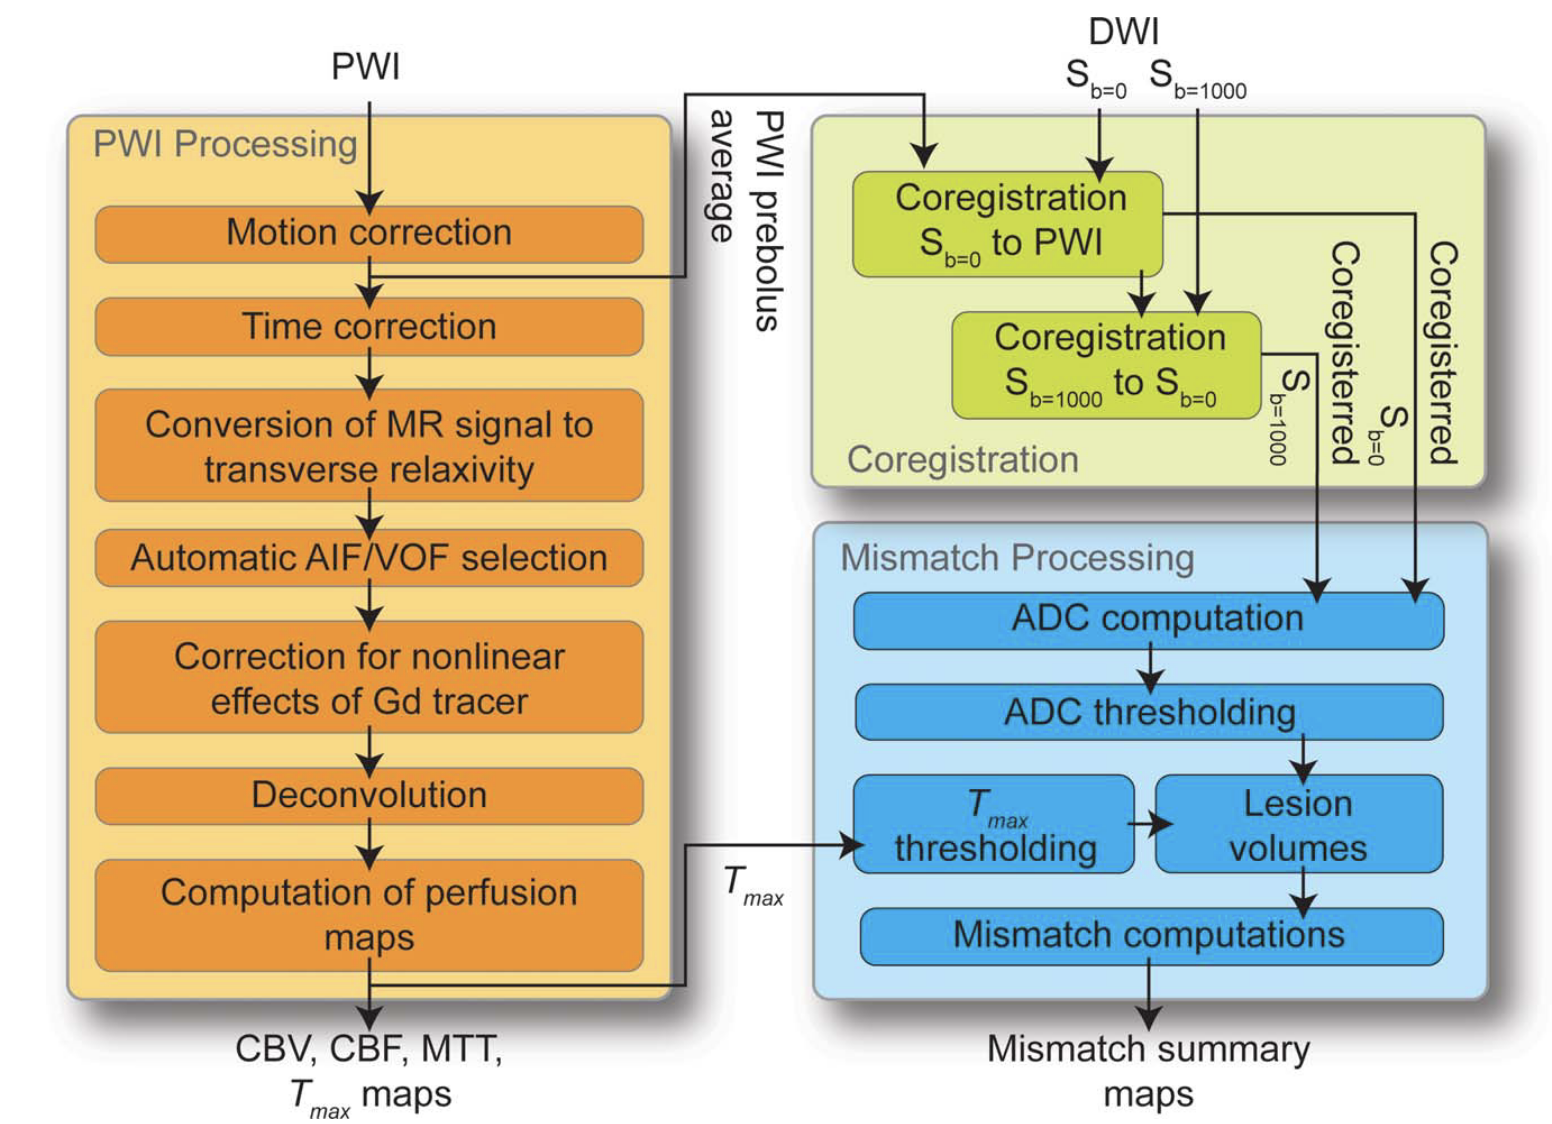
\includegraphics[width=\linewidth]{figures/intro-straka.png}
            \caption{Details of the RAPID pipeline used to calculate mismatch between DWI and PWI from \cite{strakaRealTimeDiffusion2010}.}
            \label{fig:straka}
        \end{figure}
    \end{column}
    %
    \end{columns}   %% End of multiple columns 
    % 

\end{frame}

%%% Local Variables:
%%% mode: latex
%%% TeX-master: "../topic-slide-main"
%%% End:
